% Beginn des Dokuments
%
% allgemeine Einstellungen: Schriftgrße 11pt, DIN A4, deutsches Sprachpaket
%
\documentclass[11pt, a4paper, ngerman, oneside, titlepage, parskip=half, listof=totoc, bibliography=totoc, captions=tableheading, draft]{scrreprt}

% Einbindung weiterer Pakete
% deutsche Silbentrennung
\usepackage{babel}

% Zeichencoding
\usepackage[T1]{fontenc}
\usepackage[utf8]{inputenc}
\usepackage{textcomp}
\usepackage{lmodern}
\usepackage{}

% mathematischer Formelsatz und Symbole
\usepackage{amsmath}
\usepackage{amssymb}
\usepackage{amsfonts}

% Einbinden von externen Grafiken
\usepackage{graphicx}
\usepackage{float}
\graphicspath{{images/}}
\DeclareGraphicsExtensions{.pdf,.png,.jpg}
\usepackage{subfigure}
\newcommand{\subfigureautorefname}{\figurename}

% Hyperlinks zwischen Textstellen und zu externen Dokumenten
\usepackage[pdfauthor={Daniel Probst}, pdftitle={Versuchsstand für Kleinmotoren}, pdfsubject={Aufbau und Einrichtung eines neuen Praktikumversuchs mit einer bürstenlosen Gleichstrommaschine und einem Hybrid-Schrittmotor}]{hyperref}

% Erweiterung verbatim-Umgebung für Codezeilen
\usepackage{listings}

% Tabellen über mehrere Seiten mit automatischem Seitenumbruch
%\usepackage{longtable}

% Verbesserung Tabellenfunktionen
\usepackage{array}
\usepackage{booktabs}
\usepackage{multirow}
\usepackage{tabularx}

% bessere Zeilenumbrüche
\usepackage[final]{microtype}

% Formatierung Zahlen und physikalische Einheiten
\usepackage{siunitx}

% Umlaute für BibTeX
\usepackage{babelbib}

% Kopfzeile anpassen
\usepackage[automark, headsepline, ilines]{scrpage2}
\pagestyle{scrheadings}
\clearscrheadings
\ihead{\headmark}
\ohead{\author}

% für todo und listoftodo
\usepackage[obeyDraft]{todonotes}

% eigene Befehle einbinden
% Referenz f�r Abbildung
\newcommand{\abbildung}[1]{Abbildung \ref{#1}}

% Referenz f�r Tabelle
\newcommand{\tabelle}[1]{Tabelle \ref{#1}}

% Referenz f�r Formel
\newcommand{\formel}[1]{Formel \eqref{#1}}

% Dokumententitel
\title{Versuchsstand für Kleinmotoren -- Aufbau und Einrichtung eines neuen Praktikumsversuchs mit einer bürstenlosen Gleichstrommaschine und einem Hybrid-Schrittmotor}
\author{Daniel Probst}
\date{\today, Regensburg}

\makeindex

\begin{document}

\maketitle

\pagenumbering{Roman}
\tableofcontents

\clearpage
\pagenumbering{arabic}

\chapter{Schrittmotor}

Schrittmotoren funktionieren vom Prinzip her ebenso wie die bürstenlosen Gleichstrommaschinen wie eine Synchronmaschine. Der Unterschied zu den BLDC-Maschinen liegt darin, dass bedingt durch den Aufbau eine Umdrehung in eine bestimmte Anzahl von Schritten unterteilt werden kann. Diese Anzahl lässt sich je nach Ansteuerungsart noch weiter unterteilen.

Durch die Kenntnis des zurückgelegten Winkels kann man hier auf eine Positionsregelung, welche eine Rückführung der Lage notwendig macht, verzichten, da man darauf vertraut, dass die gewollte Position eingenommen wird. Dies nennt man regelungstechnisch eine offene Steuerkette und ist auch der größte Vorteil gegenüber anderen Positionierantrieben, da eine aufwendige und somit auch teure Positionserkennung hinfällig ist.

Die offene Steuerkette bringt bei der Auslegung des Schrittantriebes jedoch auch gewisse Besonderheiten mit sich, die beachtet werden müssen. So ist der Antrieb im Allgemeinen für die auftretenden Lastmomente überzudimensionieren, da es sonst zu Schrittverlusten und im schlimmsten Fall zum Stillstand kommen kann. Weiterhin ist die maximale Drehzahl begrenzt, da, wie später noch gezeigt wird, das maximal aufbringbare Drehmoment ab einer gewissen Drehzahl stark abfällt. Die Frequenz, mit der ein Schrittmotor ohne Verlust losfahren kann, ist ebenfalls begrenzt.

In der Praxis haben sich Schrittmotoren vor allem bei leistungsarmen und drehzahlniedrigen Anwendungen durchgesetzt. Als Beispiele sind hier

\begin{itemize}
	\item Drucker
	\item CD-ROM-Laufwerke und Festplatten
	\item Positioniertische
	\item Kleinroboter
\end{itemize}

zu nennen.

Als Bauformen haben sich im Wesentlichen drei verschiedene durchgesetzt. Dies sind der PM-Schrittmotor, der Reluktanzschrittmotor und der Hybridschrittmotor. Der Aufbau sowie die Wirkungsweise dieser drei Arten von Schrittmotoren soll zunächst dargestellt werden, bevor auf die Ansteuerung, die Vermessung und Simulation des verwendeten Motors sowie einen konkreten Anwendungsfall eingegangen wird.

\section{PM-Schrittmotor}

PM-Schrittmotoren (PM steht hierbei für permanent magnet) trägt seinen Namen daher, dass der Läufer aus einem Permanentmagneten besteht. Von dieser Bauform gibt es noch einmal weitere Unterformen, genannt seien hier der Klauenpol- und der Scheibenmagnetschrittmotor. Zunächst soll die Funktionsweise anhand eines grundsätzlichen Modells erläutert , anschließend auf die konstruktionstechnischen Besonderheiten der Unterformen eingegangen werden.

\subsection{Funktionsweise}

In \abbildung{fig:PM_Schrittmotor} ist ein zweisträngiger PM-Schrittmotor mit 2 Polen nach \cite{Schroeder2007} dargestellt. Es werden die beiden Möglichkeiten für je einen erregten Strang gezeigt. So ist im linken Bild Strang A und im rechten Bild Strang B erregt. Die Positionen, die der Rotor dabei einnimmt, sind bereits gezeichnet. Zu begründen ist dies mit dem geringsten magnetischen Widerstand bei diesen Positionen. Betrachtet man das linke Bild, so erhält man unter Anwendung der Rechte-Hand-Regel im Stator oben einen Südpol und unten einen Nordpol. Der Rotor richtet sich dann danach aus. Analog verfährt man beim rechten Teilbild.

\begin{figure}[H]
\centering
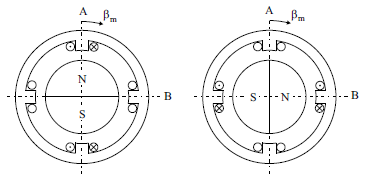
\includegraphics{PM_Schrittmotor}
\caption{Prinzippild eines zweisträngigen PM-Schrittmotors}
\label{fig:PM_Schrittmotor}
\end{figure}

Nimmt man nun an, dass immer nur ein Strang bestromt wird, so erhält man vier mögliche Rotorlagen, je nach bestromtem Strang und Richtung des Stromes. Eine solche Rotorlage nennt man beim Schrittmotor Vollschritt. Das behandelte Modell lässt sich also in vier Vollschritte unterteilen. Generell gilt für die Anzahl der Vollschritte $z$ \formel{eq:vollschritt}. Hierbei ist $p$ die Polpaarzahl des Motors und $m$ die Strangzahl.

\begin{equation}
z=2 \cdot p \cdot m
\label{eq:vollschritt}
\end{equation}

Geht man davon aus, dass im Modell oben bei Strang A der Winkel $\beta_{m}$ 0° beträgt und im Uhrzeigersinn positiv gezählt wird, was eigentlich nicht üblich ist, so können die Winkel 0°, 90°, 180° und 270° angefahren werden.

Bisher galt die Annahme, dass nur ein Strang bestromt werden kann. Dies muss allerdings nicht sein. Es können auch beide Stränge bestromt werden. Erregt man die beiden Stränge A und B zum Beispiel so, dass oben und rechts ein Südpol entsteht, dann wird aufgrund des geringsten magnetischen Widerstands der Rotor eine Lage von 45° einnehmen.

Werden nun immer zwei Stränge erregt, so erhält man wieder vier Vollschritte, diesmal allerdings mit um 45° verschobenen Winkeln. Das Drehmoment ist bei zwei bestromten Strängen allerdings höher als bei nur einem erregten Strang, da sich die Magnetfelder überlagern. Geht man davon aus, dass der Betrag der beiden Ströme gleich groß ist, so erhält man aufgrund der geometrischen Addition eine Flussdichte, die den $\sqrt{2}$-fachen Wert wie bei einem erregten Strang annimmt.

\tabelle{tab:vollschritt} zeigt die anfahrbaren Winkel des Models bei Vollschrittbetrieb \cite{Schroeder2007}. $n$ ist hierbei die Anzahl der stromdurchflossenen Stränge.

\begin{table}[H]
\centering
\caption{Winkel $\beta_{m}$ bei Vollschrittbetrieb und unterschiedlich erregten Statorsträngen}
\begin{tabular}[t]{lcccc}
\toprule
Schritt & 1 & 2 & 3 & 4 \\
\midrule
Winkel $\beta_{m}$ bei Vollschrittbetrieb und $n=1$ & 0° & 90° & 180° & 270° \\
Winkel $\beta_{m}$ bei Vollschrittbetrieb und $n=2$ & 45° & 135° & 225° & 315° \\
\bottomrule
\end{tabular}

\label{tab:vollschritt}
\end{table}

Wechselt man die Anzahl der durchflossenen Stränge ab, so nennt man das Halbschrittbetrieb. Man erhält dann die Kombination an Positionen aus \tabelle{tab:vollschritt} und somit die doppelte Anzahl Schritte wie bei Vollschrittbetrieb. Die Formel hierzu lautet

\begin{equation}

z=4\cdot p \cdot m

\label{eq:halbschritt}
\end{equation}

Allerdings erhält man hier dann ein wechselndes Drehmoment, je nachdem, ob gerade eine oder zwei Stränge bestromt werden.

Ein Vorteil des PM-Schrittmotors ist der, dass im stromlosen Zustand ein Selbsthaltemoment entsteht, wenn der Rotor aus einer Vorzugsposition ausgelenkt wird. Betrachtet man hier \abbildung{fig:PM_Schrittmotor}, so liegen die Vorzugspositionen in Richtung der horizontalen und vertikalen Achse, die Rotorausrichtung hängt dabei von der vorher angefahrenen Position ab. Das entstehen des Selbsthaltemoments lässt sich wieder mit dem geringsten magnetischen Widerstand erklären, da bei horizontaler oder vertikaler Lage der Luftspalt am geringsten ist.

\subsection{Klauenpolschrittmotor}

\subsection{Scheibenmagnetschrittmotor}

\section{Reluktanzschrittmotor}
\todo{Aufbau und Wirkungsweise}

\section{Hybridschrittmotor}
\todo{Aufbau und Wirkungsweise}

\listoffigures

\listoftables

\bibliography{literatur}{}
\bibliographystyle{babplain}
\nocite{*}

\end{document}